% Russian language
\documentclass{article}
\usepackage{geometry}
 \geometry{
 a4paper,
 total={170mm,257mm},
 left=2mm,
 top=2mm,
 }
\usepackage[utf8]{inputenc}
\usepackage[russian]{babel}

% Math symbols
\usepackage{amssymb}
\usepackage{amsmath}

% Images inplace
\usepackage{float}
\usepackage{graphicx}

% Code blocks
\DeclareFixedFont{\ttb}{T1}{txtt}{bx}{n}{12} % for bold
\DeclareFixedFont{\ttm}{T1}{txtt}{m}{n}{12}  % for normal
\usepackage{color}
\definecolor{deepblue}{rgb}{0,0,0.5}
\definecolor{deepred}{rgb}{0.6,0,0}
\definecolor{deepgreen}{rgb}{0,0.5,0}
\usepackage{listings}
\newcommand\pythonstyle{\lstset{
language=Python,
basicstyle=\ttm,
morekeywords={self},              % Add keywords here
keywordstyle=\ttb\color{deepblue},
emph={MyClass,__init__},          % Custom highlighting
emphstyle=\ttb\color{deepred},    % Custom highlighting style
stringstyle=\color{deepgreen},
frame=tb,                         % Any extra options here
showstringspaces=false
}}
\lstnewenvironment{python}[1][]
{
\pythonstyle
\lstset{#1}
}
{}
\newcommand\pythonexternal[2][]{{
\pythonstyle
\lstinputlisting[#1]{#2}}}
\newcommand\pythoninline[1]{{\pythonstyle\lstinline!#1!}}
% Code blocks


\title{Лабораторная работа №3}
\author{Ларин Егор. 4 группа 2 курс}

\begin{document}
\maketitle
\section*{Теория}

\begin{equation*}
    N= 10, a = -2, b=2, h = \frac{b-a}{N}, f(x) = e ^ {\cos x}, f'(x) = -\sin(x) e^{\cos x}
\end{equation*}



\begin{equation*}
    \begin{cases}
        \frac{h}{6} M_{i-1} + \frac{2h}{3} M_i + \frac{h+1}{6} M{i+1} = \frac{f_{i+1} - f_i}{h} - \frac{f_i - f{i-1}}{h}, i = \overline{2, N-2}\\
        \frac{h}{3}M_0 + \frac{h}{6} M_1 = \frac{f_1 - f_0}{h} - f'(a)\\
        \frac{h}{3}M_N + \frac{h}{6} M_{N-1} = \frac{f_{N-1} - f_N}{h} + f'(b)\\
    \end{cases}
\end{equation*}

\begin{equation*}
    S_3(x) = \left\{ P{i,3}(x) = M_{i-1} \frac{(x_i - x)^3}{6h} + M_i \frac{(x-x_{i-1})^3}{6h} + (f_{i-1} - \frac{h_i^2}{6} M_{i-1} )\frac{x_i -x}{h} + (f_i - \frac{h^2}{6} M_i)\frac{x-x_{i-1}}{h} \\| x \in \left[ x_{i-1}, x_i \right], i = \overline{1, N} \right\}
\end{equation*}

\section*{Листинг кода}
\begin{python}
from math import exp, cos, sin
import numpy as np
from matplotlib import pyplot as plt

a = -2
b = 2
N = 10
h = (b-a) / N
f = lambda x: exp(cos(x))
dfdx = lambda x: -sin(x) * exp(cos(x))
# f = lambda x: abs(x)
# dfdx = lambda x: -1 if x== -2 else 1
xss = [a + i*h for i in range(0, N+1)]
yss = [f(x) for x in xss]

def TDMA(a, b, c, d):
    n = len(d)
    w=  [.0] * (n-1)
    g= [.0] * n
    p= [.0] * n
    
    w[0] = c[0]/b[0]
    g[0] = d[0]/b[0]

    for i in range(1,n-1):
        w[i] = c[i]/(b[i] - a[i-1]*w[i-1])
    for i in range(1,n):
        g[i] = (d[i] - a[i-1]*g[i-1])/(b[i] - a[i-1]*w[i-1])
    p[n-1] = g[n-1]
    for i in range(n-1,0,-1):
        p[i-1] = g[i-1] - w[i-1]*p[i]
    return p

css = []
ass = []
bss = []
dss = []
for i in range(0, N+1):
    if i== 0:
        ass.append(h/3)
        bss.append(h/6)
        dss.append((yss[1] - yss[0])/h - dfdx(a))
    elif i== N:
        css.append(h/6)
        ass.append(h/3)
        dss.append(dfdx(b) - (yss[N] - yss[N-1])/h)
    else:
        css.append(h/6)
        ass.append(2*h/3)
        bss.append(h/6)
        dss.append((yss[i+1] - yss[i])/h - (yss[i] - yss[i-1])/h)

mss = TDMA(css,ass,bss,dss)
sss = []

def wrap(i):
    def s(x): 
        return (xss[i] - x)**3 * mss[i-1] / (6*h)  + (x-xss[i-1])**3 * mss[i] / (6*h) + (yss[i-1] - mss[i-1]*h*h/6)*(xss[i] - x)/h + (yss[i] - mss[i] *h*h /6)*(x-xss[i-1])/h
    return s

for i in range(1, N+1):
    sss.append(wrap(i))

def S(x):
    i  = int((x - a)/h)
    if i == 10:
        i = 9
    return sss[i](x)

def compare(n):
    d = (b-a)/n
    xs = [a + i * d for i in range(n+1)]
    plt.plot(
            xs, [S(x) for x in xs], "b",
            xs, [f(x) for x in xs],  "r",
            xss, [f(x) for x in xss], "ro",
    )
    plt.legend(["S(x)", "f(x)"])
    plt.show()

def error():
    d = (b-a)/100
    xs = [a + i * d for i in range(101)]
    return max([abs(f(x) - S(x)) for x in xs])

print(error())
compare(100)
\end{python}

\section*{Результаты численного эксперимента}

\subsection*{Оценка погрешности}
\begin{equation*}
    max_{i=0,100} \left|S_3(\overline{x_i} - f(\overline{x_i}) \right| = 0.0008154280452394858
\end{equation*}
\subsection*{График}
\begin{figure}[H]
\caption{}
\centering
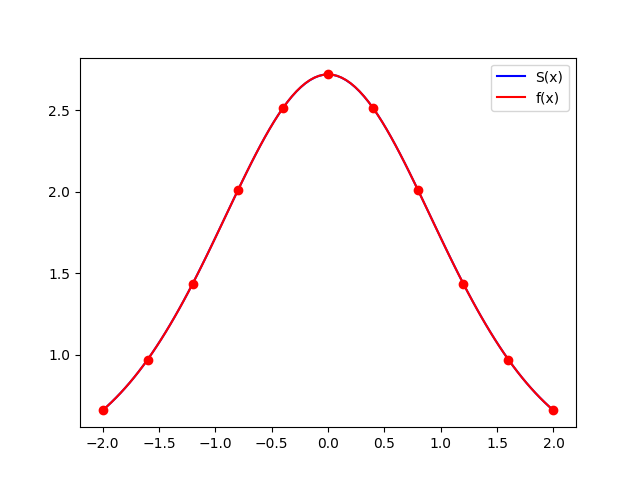
\includegraphics[width=0.9\textwidth]{figure}
\end{figure}

\section*{Выводы}
Кубический сплайн хорошо приближает функции с непрерывной производной.
\end{document}